%!TEX program = lualatex
\documentclass[12pt, a4paper]{article}

\usepackage{fontspec}
\setmainfont[
  Ligatures=TeX,
  Path=/usr/share/texmf/fonts/opentype/public/tex-gyre/,
  UprightFont=texgyrepagella-regular.otf,
  BoldFont=texgyrepagella-bold.otf,
  ItalicFont=texgyrepagella-italic.otf,
  BoldItalicFont=texgyrepagella-bolditalic.otf
]{TeX Gyre Pagella}
\usepackage{microtype}
\usepackage{amsmath, amssymb, amsthm}
\usepackage{geometry}
\usepackage{setspace}
\usepackage{titlesec}
\usepackage{hyperref}
\usepackage{xcolor}
\usepackage{booktabs}
\usepackage{mathtools}
\usepackage{tikz}
\usetikzlibrary{arrows.meta, positioning, calc}
\usepackage{fancyhdr}
\usepackage{emptypage}
\usepackage{natbib}

\geometry{
  a4paper,
  top=2.8cm, bottom=3cm,
  left=3.2cm, right=3.2cm,
  headheight=14pt
}

\definecolor{rsvpblue}{HTML}{1A2E4A}
\definecolor{accentgold}{HTML}{8B6914}
\definecolor{midgray}{HTML}{555555}
\definecolor{lightgray}{HTML}{AAAAAA}

\hypersetup{
  colorlinks=true,
  linkcolor=rsvpblue,
  citecolor=accentgold,
  urlcolor=midgray
}

\pagestyle{fancy}
\fancyhf{}
\fancyhead[LE,RO]{\small\color{lightgray}\thepage}
\fancyhead[RE]{\small\color{lightgray}\itshape HYDRA: Architecture, Geometry, and the Problem of Coherent Agency}
\fancyhead[LO]{\small\color{lightgray}\itshape\leftmark}
\renewcommand{\headrulewidth}{0pt}

\titleformat{\section}{\large\bfseries\color{rsvpblue}}{\thesection.}{0.8em}{}
\titleformat{\subsection}{\normalsize\bfseries\color{midgray}}{\thesubsection.}{0.6em}{}
\titlespacing{\section}{0pt}{2.4ex plus 0.5ex}{1.1ex}
\titlespacing{\subsection}{0pt}{1.6ex plus 0.3ex}{0.6ex}

\newtheoremstyle{rsvpstyle}
  {8pt}{8pt}{\itshape}{0pt}{\bfseries\color{rsvpblue}}{.}{0.5em}{}
\theoremstyle{rsvpstyle}
\newtheorem{theorem}{Theorem}[section]
\newtheorem{proposition}[theorem]{Proposition}
\newtheorem{lemma}[theorem]{Lemma}
\newtheorem{corollary}[theorem]{Corollary}

\theoremstyle{definition}
\newtheorem{definition}[theorem]{Definition}
\newtheorem{conjecture}[theorem]{Conjecture}
\newtheorem{remark}[theorem]{Remark}

\setstretch{1.18}
\setlength{\parskip}{0.45em}
\setlength{\parindent}{1.5em}

\newcommand{\Traj}{\mathcal{X}}
\newcommand{\OpMan}{\mathcal{M}}
\newcommand{\Adm}{\mathcal{A}}
\newcommand{\ProjFam}{\Pi}
\newcommand{\Persist}{P}
\newcommand{\Real}{\mathcal{R}}
\newcommand{\AF}[1]{A(#1)}
\newcommand{\Hol}{\mathrm{Hol}}

\begin{document}

%% ══════════════════════════════════════════════════════════
\begin{titlepage}
\thispagestyle{empty}
\vspace*{3.5cm}
\begin{center}
{\huge\bfseries\color{rsvpblue} HYDRA\\[0.6em]}
{\large\bfseries\color{midgray}
Architecture, Geometry, and the\\[0.3em]
Problem of Coherent Agency
}
\vspace{2.8cm}

{\large Flyxion}\\[0.3em]
{\small\color{midgray} Independent Researcher}

\vspace{1.8cm}
{\small\color{midgray}
\begin{minipage}{0.78\textwidth}
\centering\itshape
A critical reconstruction tracing the development of HYDRA from a
hybrid cognitive architecture (2025) through a geometric theory of admissible
computation (2026), incorporating the full source texts and situating the
framework within the RSVP--MEM\textbar8--Simulated Agency research program.
\end{minipage}
}
\vspace{4cm}
{\small\color{midgray} 2026}
\end{center}
\end{titlepage}

%% ══════════════════════════════════════════════════════════
\clearpage
\thispagestyle{empty}
\vspace*{2cm}
\begin{center}{\bfseries\color{rsvpblue} Abstract}\end{center}
\noindent
HYDRA (Hybrid Dynamic Reasoning Architecture) originated in 2025 as a practical
AI architecture synthesizing PERSCEN's personalized feature graphs, Relevance
Activation Theory's cue-driven gradient flows, Chain of Memory's differentiable
latent stack, and RSVP/TARTAN's field-theoretic semantic representations into
a unified reasoning pipeline. By 2026 the same six-component composition had
been reinterpreted as a compositional geometric system over stratified semantic
manifolds, with the engineering modules recast as functorial operators, the
reasoning pipeline as a proof-carrying dependent type, and the memory layer as
stabilized field residue governed by Lyapunov dynamics. This document traces
that development in full, presenting the mathematics of both incarnations,
the critical synthesis connecting them, and twelve appendices collecting
the supporting formal machinery. Standard mathematical results are distinguished
from framework-specific definitions and open conjectures by context and citation.
The Structural Universality result is stated explicitly as a conjecture throughout.
All references are to the mathematical, physical, and cognitive-scientific
literature from which the formal machinery is drawn.

\tableofcontents
\clearpage

%% ══════════════════════════════════════════════════════════
\section{Three Stages of Development}
%% ══════════════════════════════════════════════════════════

HYDRA did not arrive fully formed as a geometric ontology. Its development
passes through three recognizable stages, each preserving the same six
architectural components while progressively reinterpreting their significance.

In its earliest formulation HYDRA is a cognitive architecture. The primary
concerns are interpretability, personalization, memory, and reasoning in AI
agents, and the framework is positioned alongside recommender systems,
robotics, and safety-critical AI. The six components are engineering modules
whose correctness is evaluated against task performance. The core pipeline is:
\begin{equation}\label{eq:pipeline}
  H \;=\; \mathrm{GLU}_{\mathrm{RSVP}} \circ M \circ T \circ F_a \circ G_a \circ R
\end{equation}
where $R$ maps cues to relevance fields, $G_a$ constructs personalized graphs,
$F_a$ maps graphs to representations, $T$ tiles semantic space recursively,
$M$ supplies latent memory trajectories, and $\mathrm{GLU}_{\mathrm{RSVP}}$ is
the entropy-constrained gating layer \citep{MacLane1998}.

The second stage reinterprets the pipeline geometrically. The important object
is no longer a representation but a path through a constrained manifold.
Semantic equivalence ceases to be defined by symbolic similarity and is
instead defined through identical admissible future continuations. The Minimal
Projection Theorem (Section~\ref{sec:minproj}) formalizes this shift.

The third stage treats the same mathematical structures as recurring invariants
across cognition, software, memory, infrastructure, economics, and cosmology.
The invariant object is not intelligence itself but organized persistence under
admissibility constraints. The Structural Universality Conjecture
(Section~\ref{sec:universality}) is the culminating claim of this stage.

What changes across all three stages is interpretation, not architecture.
The architectural skeleton is stable; the ontology deepens.

%% ══════════════════════════════════════════════════════════
\section{Four Primitive Objects}
\label{sec:primitives}
%% ══════════════════════════════════════════════════════════

Almost everything in this document is a specialization of four mathematical
primitives. Introducing them here, before the specific field equations and
engineering details, gives the remaining sections a common reference point.
Each later section can be understood as: here is how the four primitives
specialize in this domain.

\begin{definition}[Trajectory Space]
A \emph{trajectory space} $\Traj$ is a topological space of agent-environment
histories, equipped with an admissibility structure $\Adm \subset \Traj$ and
a measure $\mu$.
\end{definition}

\begin{definition}[Projection System]
A \emph{projection system} $\ProjFam = \{\pi_i : \Traj \to \OpMan_i\}$ is a
family of continuous surjections onto lower-dimensional operational manifolds,
satisfying mutual consistency on overlapping domains \citep{TenenbaumSilvaLangford2000}.
\end{definition}

\begin{definition}[Admissibility Structure]
An \emph{admissibility structure} $\Adm$ specifies permitted transitions.
A state $x$ is admissible relative to trajectory $\gamma$ if it lies in the
closure of $\Adm$-preserving transitions from the current position along $\gamma$.
Admissibility is relational: a state is not admissible in isolation but
relative to a trajectory and a family of allowed continuations.
\end{definition}

\begin{definition}[Persistence Functional]
A \emph{persistence functional} $\Persist(\Traj, \ProjFam, \Adm)$ is a
Lyapunov-type functional measuring the degree to which the projection system
preserves admissibility under the field dynamics \citep{Arnold1989}.
\end{definition}

\begin{remark}
RSVP cosmology, HYDRA cognition, MEM\textbar8 memory, Semantic Infrastructure,
Yarncrawler, and the political economy of platform extraction are all
specializations of $(\Traj, \ProjFam, \Adm, \Persist)$. Section~\ref{sec:universality}
makes this claim precise; it remains a conjecture pending categorical formalization.
\end{remark}

%% ══════════════════════════════════════════════════════════
\section{The Minimal Projection Theorem}
\label{sec:minproj}
%% ══════════════════════════════════════════════════════════

The following is the conceptual center of the entire document. It appears under
different names throughout the broader research program and is the result from
which projection collapse, semantic equivalence, fiber structure, and the
universality conjecture all descend.

\begin{definition}[Admissibility Projection]
An \emph{admissibility projection} is a smooth map $\pi : \Traj \to \OpMan$
satisfying: $A(x_1) = A(x_2) \Rightarrow \pi(x_1) = \pi(x_2)$.
\end{definition}

\begin{theorem}[Existence of Minimal Projection]
\label{thm:minproj}
For any trajectory space $\Traj$ with admissibility relation $A$, there
exists a minimal admissibility projection $\pi^* : \Traj \to \OpMan^*$,
unique up to isomorphism, such that every other admissibility projection
factors through $\pi^*$ \citep{Hatcher2002,MacLane1998}.
\end{theorem}

\begin{proof}
Define $x_1 \sim x_2 \Leftrightarrow A(x_1) = A(x_2)$. This is an equivalence
relation by reflexivity, symmetry, and transitivity of set equality. Set
$\OpMan^* = \Traj/{\sim}$ and $\pi^*(x) = [x]_\sim$. For any other
admissibility projection $\pi$, define $\bar\pi([x]_\sim) = \pi(x)$;
well-definedness follows from the admissibility projection condition. The
universal property of quotients gives the factorization and uniqueness.
\end{proof}

\begin{definition}[Semantic Equivalence]
States $x_1, x_2 \in \Traj$ are \emph{semantically equivalent} iff
$A(x_1) = A(x_2)$: identical future admissible continuation structure.
Meaning is relational and context-dependent rather than intrinsic.
\end{definition}

\begin{remark}
Theorem~\ref{thm:minproj} is the core established result. All subsequent
claims about projection collapse, semantic fibers, meritocratic hubris, and
hallucination obstruction are applications of the same quotient construction
to different admissibility structures. The theorem itself is standard
mathematics; the applications are framework-specific or conjectural.
\end{remark}

%% ══════════════════════════════════════════════════════════
\section{The 2025 Architecture}
%% ══════════════════════════════════════════════════════════

The original HYDRA proposal integrates four distinct frameworks:
PERSCEN's user-specific feature graph modeling, Relevance Activation Theory
for cue-driven gradient-based cognition, Chain of Memory for causally faithful
latent memory trajectories, and RSVP/TARTAN for recursive field-theoretic
semantic representations \citep{Friston2010}. The six components of
equation~\eqref{eq:pipeline} are presented here as they appeared in 2025,
before the geometric reinterpretation. Readers already familiar with the
architecture may proceed to Section~\ref{sec:rsvp}.

\subsection{Cue Activation Layer}

Each cue $c \in C$ maps to a Gaussian relevance field:
\begin{equation}
  \rho_c(x) = \exp\!\Bigl(-\tfrac{1}{2}(x-\mu_c)^\top\Sigma_c^{-1}(x-\mu_c)\Bigr)
\end{equation}
The induced gradient flow $\dot{x} = \nabla\rho_c(x)$ governs attention and behavior.
The functor $R : \mathbf{Top} \to \mathbf{Field}$ maps cues to fields.

\subsection{Personalized Feature Graph}

For each agent $a$, adjacency matrix:
$[A_a^{(1)}]_{m,:} = \mathrm{MLP}_m([e_{a,1},\ldots,e_{a,N_f},\mathrm{one\text{-}hot}(m)])$.
A GNN computes higher-order interactions; $G_a : \mathbf{Cue} \to \mathbf{Graph}$
encodes personalized semantic neighborhood structure \citep{ZhangEtAl2020}.

\subsection{Recursive Scene Memory and TARTAN}

Tiles $T_i = \{x \in \Omega \mid S_i(x) < \tau_i\}$ with aura fields
$\alpha_i(x) = (\Phi_i(x), v_i(x), S_i(x))$ and recursive refinements
$T_i^{(k+1)} = T_i^{(k)} \cap \{x \mid S_i^{(k+1)}(x) < \tau_i^{(k+1)}\}$.

\subsection{Latent Memory Stack}

Memory states $M_{i+1} = \phi(M_i, u_i, c_i)$ with causal influence traced by
$\mathcal{I}(M_i \to y) = \|\partial y/\partial M_i\|$ \citep{Pearl2009}.

\subsection{Progressive Reasoning Core}

Entropy consistency is enforced via
$dS/dt = -\gamma\int_\Omega\|\nabla S\|^2\,dx$.
The adjoint constraint $\langle v\cdot\nabla\Phi, \psi\rangle = \langle\Phi,
-\nabla\cdot(v\psi)\rangle$ gives $\mathrm{GLU}_{\mathrm{RSVP}}(x,y) =
\sigma(Ax + B\Phi) \odot (Cy + D(\nabla\cdot v))$. Memory curvature update:
$M_{i+1} = M_i + \Delta t(v_M - \lambda R(X,Y)v_M)$ stabilizes ambiguous regions
\citep{Lee2013}.

%% ══════════════════════════════════════════════════════════
\section{RSVP as an Ontology of Admissible Fields}
\label{sec:rsvp}
%% ══════════════════════════════════════════════════════════

The RSVP field triple is the primary realization of the four primitive objects
in the field-theoretic setting. Understanding RSVP is necessary for the memory,
stratification, and sheaf sections that follow.

\begin{definition}[RSVP Field Triple]
The RSVP field triple over smooth manifold $\OpMan$ is $(\Phi, v, S)$ where
$\Phi : \OpMan\times\mathbb{R}\to\mathbb{R}$ is the scalar accessibility
potential, $v : \OpMan\times\mathbb{R}\to T\OpMan$ is the vector flow field,
and $S : \OpMan\times\mathbb{R}\to\mathbb{R}$ is the entropic accessibility
measure $S(x,t) = \log|A(x,t)|$.
\end{definition}

The RSVP field equations are novel, but their structure is inspired by coupled
wave-diffusion systems in field theory and nonlinear dynamics
\citep{Arnold1989,Tao2016}:
\begin{align}
  \Box\Phi + \mu^2\Phi &= \rho(v,S) \label{eq:scalar}\\
  \nabla_\OpMan \cdot v &= -\tfrac{\partial S}{\partial t} \label{eq:div}\\
  \tfrac{\partial S}{\partial t} + v\cdot\nabla_\OpMan S &= \sigma(\Phi,v) \label{eq:entropy}
\end{align}
The source terms $\rho$ and $\sigma$ are not derived from first principles here;
their derivation for specific domains is an open problem (Section~\ref{sec:open}).
Equation~\eqref{eq:div} is a continuity equation: diverging flow loses
admissibility; converging flow gains it.

\begin{proposition}[Lyapunov Stability of Admissibility Maxima]
\label{prop:lyap}
If $x^*$ is an isolated local maximum of $\Phi(\cdot,t)$ and
$v = \alpha\nabla\Phi + \xi$ with $\alpha > 0$ and $\|\xi\|$ small, then $x^*$
is Lyapunov stable for the flow of $v$ \citep{Arnold1989}.
\end{proposition}

\begin{proof}
$L(x) = \Phi(x^*) - \Phi(x) \geq 0$ is a Lyapunov function. Near $x^*$ the
Hessian is negative definite; when $\|\xi\|$ is small relative to
$\alpha\|\nabla\Phi\|$, $\dot{L} < 0$ in a punctured neighborhood of $x^*$.
\end{proof}

\begin{remark}
This proposition uses established Lyapunov theory applied to RSVP
dynamics. Its conclusion --- that local maxima of $\Phi$ are attractors ---
holds whenever $v \approx \alpha\nabla\Phi$. Whether the full RSVP equations
\eqref{eq:scalar}--\eqref{eq:entropy} produce such flow globally is part of the
regularity problem listed in Section~\ref{sec:open}.
\end{remark}

%% ══════════════════════════════════════════════════════════
\section{Stratified Semantic Manifolds}
%% ══════════════════════════════════════════════════════════

This section is built on genuine established mathematical machinery and is
the most rigorously grounded part of the framework.

\begin{definition}[Whitney Stratification]
A Whitney stratification of $\OpMan \subseteq \mathbb{R}^n$ is a partition
$\OpMan = \bigsqcup_\alpha S_\alpha$ into locally closed smooth submanifolds
satisfying the frontier condition and Whitney condition B: for sequences
$y_k \to p$ in $S_\beta$ and $x_k \to p$ in $S_\alpha$, if secants
$\overrightarrow{y_kx_k} \to \ell$ and tangent spaces $T_{x_k}S_\alpha \to \tau$,
then $\ell \subseteq \tau$ \citep{Whitney1965,Mather1973}.
\end{definition}

\begin{definition}[Tangent-Constrained Gradient]
For $F : \OpMan \to \mathbb{R}$ and $x \in S_\alpha$, the tangent-constrained
gradient is $\nabla_{S_\alpha}F(x) = \Pi_{T_xS_\alpha}(\nabla F(x))$
\citep{Lee2013}.
\end{definition}

\begin{theorem}[Convergence of Tangent-Constrained Gradient Descent]
\label{thm:tcgd}
Let $F : S_\alpha \to \mathbb{R}$ be $L$-smooth and $\mu$-strongly convex.
Then tangent-constrained gradient descent with $\eta \in (0, 2/L)$ converges
to the minimizer at geometric rate $\bigl(1 - 2\eta\mu(1-\eta L/2)\bigr)^t$
\citep{Lee2013}.
\end{theorem}

\begin{theorem}[TARTAN Approximation]
\label{thm:tartan}
For any $\epsilon > 0$ and compact $K \subseteq \OpMan$ with finitely many
strata, there exists a finite tile decomposition with noise annotation
$\eta(T_i) \leq \epsilon$ for all tiles, by the uniform continuity of smooth
functions on compact strata and a finite subcover argument \citep{Whitney1965}.
\end{theorem}

\begin{remark}
Theorem~\ref{thm:tartan} uses only uniform continuity and compactness.
The identification of tiles with semantic regimes is a framework interpretation that gives the theorem its cognitive significance.
\end{remark}

%% ══════════════════════════════════════════════════════════
\section{Sheaf-Theoretic Semantics}
%% ══════════════════════════════════════════════════════════

\begin{definition}[Semantic State Presheaf]
The semantic state presheaf $\mathcal{F}$ over $\mathbf{Ctx}$ assigns to each
open $U \subseteq \OpMan$ the set $\mathcal{F}(U)$ of admissible local RSVP
field configurations satisfying the field equations on $U$ with compatible
boundary conditions \citep{Godement1958}.
\end{definition}

\begin{theorem}[Semantic State Sheaf Existence]
\label{thm:sheaf}
\emph{Assuming} the RSVP field equations satisfy unique continuation on $\OpMan$
(a solution on $U$ is uniquely determined by its restriction to any non-empty
$V \subseteq U$), the semantic state presheaf $\mathcal{F}$ is a sheaf
\citep{Godement1958}.
\end{theorem}

\begin{proof}
Identity axiom: if $\rho_{U,U_i}(s) = \rho_{U,U_i}(s')$ for all $i$, unique
continuation forces $s = s'$. Gluing: sections agreeing on overlaps define a
section on the union; the field equations are satisfied locally hence globally.
\end{proof}

\begin{remark}
The assumption of unique continuation for the full non-linear RSVP system
\eqref{eq:scalar}--\eqref{eq:entropy} has not been established. This theorem
is: the sheaf construction is standard; its applicability to RSVP
fields is conditional on a regularity result that is currently open.
Unique continuation is known for linear wave equations and some semi-linear
cases \citep{Tao2016} but requires verification for the RSVP system.
\end{remark}

\begin{definition}[Hallucination as Cohomological Failure]
A system output is a \emph{hallucination} if it presents a globally
coherent-looking semantic state that is not a genuine global section of
$\mathcal{F}$. The obstruction is the \v{C}ech class
$[c] \in \check{H}^1(\mathcal{U}, \mathcal{F})$ \citep{Hatcher2002}.
\end{definition}

\begin{remark}
This definition is. The cohomological formulation of hallucination
is a research direction, not an established result. Verifying that language
model failures instantiate non-trivial $\check{H}^1$ classes in any precisely
defined semantic state sheaf would require specifying the sheaf explicitly
from model internals, which has not been done.
\end{remark}

The failure mode hierarchy ordered by cohomological character:

\begin{center}
\begin{tabular}{ll}
\toprule
\textbf{Failure mode} & \textbf{Geometric characterization} \\
\midrule
Local coherence without global coherence & $s_i$ exist but do not glue \\
Disconnected global coherence & $\OpMan$ not connected \\
Obstruction to section construction & $[c] \neq 0$ in $H^1(\OpMan,\mathcal{F})$ \\
Holonomy-induced memory distortion & parallel transport rotates section \\
Persistent cognitive conflict & $[c]$ has infinite order \\
\bottomrule
\end{tabular}
\end{center}

%% ══════════════════════════════════════════════════════════
\section{Memory as Stabilized Field Residue}
%% ══════════════════════════════════════════════════════════

\begin{theorem}[Memory Persistence Bound]
\label{thm:persist}
Suppose RSVP dynamics near memory support $K_m$ satisfy $\frac{d}{dt}\|e(t)\| \leq -\lambda\|e(t)\| + \kappa\|S\|_{L^\infty}$ with $\lambda > \kappa c_S$. Then:
\begin{equation}
  T_m \;\geq\; \frac{1}{\lambda - \kappa c_S}\log\frac{\|\Phi_m - \Phi_0\|_{L^2}}
  {\Phi_\mathrm{thresh}|K_m|^{1/2}}
\end{equation}
by the Grönwall inequality \citep{Arnold1989}.
\end{theorem}

\begin{remark}
The persistence bound is: the Grönwall argument is standard, but
the decay hypothesis on the RSVP dynamics is assumed rather than derived. It
holds when the memory excitation is sufficiently strong relative to entropic
pressure; whether RSVP field dynamics generically produce this regime is part
of the open regularity problem.
\end{remark}

Retrieval is resonance:
\begin{equation}
  \Phi_\mathrm{ret}(x) = \sum_m w_m\,\Phi_m(x),\quad
  w_m = \frac{\langle f_{c^*}, \Phi_m\rangle_{L^2}}{\sum_{m'}\langle f_{c^*},\Phi_{m'}\rangle_{L^2}}
\end{equation}
This reconstruction process resembles attractor-based recovery in neural
field theory \citep{WilsonCowan1972}.

\begin{theorem}[Resonance Retrieval as Approximate Sheaf Gluing]
\label{thm:resonance}
When stored memory fields span a dense subspace of $\mathcal{F}(\OpMan)$ in
$L^2$, the resonance superposition converges to the true global section with
error $\|\hat{s}-s\| \leq C\rho^{-\alpha}$ controlled by memory basis density
$\rho$ \citep{Rudin1991}.
\end{theorem}

\begin{remark}
This theorem is: a research direction rather than a current result. It
requires (i) the sheaf existence theorem (which depends on unique continuation,
itself unproved for RSVP), and (ii) density of the memory basis in
$\mathcal{F}(\OpMan)$, an assumption whose verification depends on the learning
dynamics. The error bound is a standard approximation result that becomes
meaningful only when these preconditions are established.
\end{remark}

\begin{theorem}[RSVP Memory as Generalized Memoization]
The RSVP memory state associated to a trajectory equivalence class $[\gamma]_\sim$
is the RSVP field configuration determined by the admissibility structure of
the class. Memoization is the field-theoretic lift of computational memoization:
the memo table is a discretized admissibility sheaf; cache reuse corresponds
to dynamic equivalence of initial conditions \citep{Bellman1957}.
\end{theorem}

\begin{remark}
The identification of memoization with admissibility-class
residue is a formal analogy, not a derivation. It is structurally correct ---
both memoization and RSVP storage depend on an equivalence relation on
trajectories --- but the analogy has not been made precise enough to yield
new computational predictions.
\end{remark}

%% ══════════════════════════════════════════════════════════
\section{Category Theory and Admissible Computation}
%% ══════════════════════════════════════════════════════════

This section is largely definitional: it establishes that the HYDRA components
are functors and gives categorical language for compositional properties.
The theorems here are reformulations of the architecture in categorical terms
rather than independently surprising results.

\begin{definition}[Category of Admissible States]
$\mathbf{AdmSt}$ has objects $(x, \Phi(x), v(x))$ for $x \in \OpMan$ and
morphisms admissible trajectories between them; composition is concatenation
\citep{MacLane1998}.
\end{definition}

The six HYDRA component functors (each):
\begin{align*}
  R &: \mathbf{Cue} \to \mathbf{Field} & G_a &: \mathbf{Field} \to \mathbf{Graph} &
  F_a &: \mathbf{Graph} \to \mathbf{Rep}\\
  T &: \mathbf{Rep} \to \mathbf{Traj}_\Adm &
  M &: \mathbf{Traj}_\Adm \to \mathbf{Mem} &
  \mathrm{GLU} &: \mathbf{Mem} \to \mathbf{Out}
\end{align*}

\begin{theorem}[Functoriality of $H$]
\label{thm:functor}
If each component is a functor preserving admissibility, then $H$ \eqref{eq:pipeline}
is a functor from $\mathbf{Cue}$ to $\mathbf{Out}$ \citep{MacLane1998}.
\end{theorem}

\begin{remark}
This is: the claim that each component is admissibility-preserving is the
framework's definition of a valid component, not a consequence derived from
other axioms. Verifying it for any concrete implementation requires showing the
implementation preserves the chosen admissibility structure.
\end{remark}

Natural transformations between HYDRA functors represent reasoning regime changes;
the naturality condition ensures that regime changes commute with contextual
specialization \citep{EilenbergMacLane1945}.

%% ══════════════════════════════════════════════════════════
\section{The Geometry of Intelligence}
%% ══════════════════════════════════════════════════════════

\begin{definition}[Coherent Agent]
A coherent agent is a system with $(\OpMan, \Phi, v, S, \pi)$ satisfying:
(i) admissible trajectory preservation; (ii) entropy regulation
$S(x(t),t) \leq S_\mathrm{max}$; (iii) local-to-global sheaf consistency;
and (iv) memory stabilization in RSVP basins.
\end{definition}

\begin{theorem}[Recursive Admissibility Stabilization]
\label{thm:ras}
A coherent agent starting from $x_0 \in \Adm_0$ and taking only
$\Adm$-preserving transitions satisfies $x_t \in \Adm_t$ for all $t \geq 0$.
\end{theorem}

\begin{proof}
By induction. Base case: $x_0 \in \Adm_0$. Inductive step: if $x_t \in \Adm_t$,
the admissible trajectory preservation condition gives $\pi(x_t) \in A(x_t)$,
and by definition of $\Adm$-preserving transitions $x_{t+1} \in \Adm_{t+1}$.
\end{proof}

\begin{remark}
This theorem is: the inductive argument is elementary; the
content depends entirely on the definition of $\Adm$-preserving transitions. It is a tautology relative to the definitions unless one imposes
independent conditions on what counts as an $\Adm$-preserving transition.
Its value is organizational: it clarifies what properties a valid implementation
must verify.
\end{remark}

The geometry-intelligence correspondence identifies: $\Phi$ with semantic
salience; $v$ with semantic tendency; $S$ with semantic ambiguity; cognition
with transport through admissibility manifolds; memory with stabilized field
residue; reasoning with local-to-global sheaf compatibility; learning with
tangent-constrained optimization; and intelligence with recursive admissibility
preservation.

%% ══════════════════════════════════════════════════════════
\section{Semantic Fibers and Agency Projection}
%% ══════════════════════════════════════════════════════════

\begin{theorem}[Realization Fibration]
\label{thm:fibration}
Under mild regularity (specifically, that $\eta \in \mathcal{N}$ is a regular
value of $\Real$), the fiber $\Real^{-1}(\eta)$ is a smooth submanifold of
$\Theta$ of codimension $\dim\mathcal{N}$, by the regular level set theorem
\citep{Lee2013,Hatcher2002}. The realization map is a Hurewicz fibration
under the further assumption that $\Real$ is a proper submersion.
\end{theorem}

\begin{remark}
The first part is (regular level set theorem). The characterization of
$\Real$ as a fibration is: it depends on $\Real$ being a proper
submersion, which must be verified for any concrete realization map.
\end{remark}

Agency projection is the identification $\OpMan \equiv \Traj$, collapsing
fibers to points. The pathology is structural: causal history information
becomes irrecoverable \citep{Pearl2009}. The ontological compression funnel
$\Traj \xrightarrow{q} \OpMan \xrightarrow{\Real} \mathcal{N}$ makes explicit
that behavioral observation is always a double projection. The same
geometric error underlies:

\begin{center}
\begin{tabular}{ll}
\toprule
\textbf{Domain} & \textbf{Manifestation of projection collapse} \\
\midrule
AI anthropomorphism & behavioral output mistaken for genuine belief \\
Social-media identity collapse & profile mistaken for person \\
Metric fixation & measure mistaken for the measured \\
Goodhart effects & proxy optimization destroying target \\
Economic legibility failures & legibility map mistaken for economy \\
\bottomrule
\end{tabular}
\end{center}

%% ══════════════════════════════════════════════════════════
\section{The Structural Universality Conjecture}
\label{sec:universality}
%% ══════════════════════════════════════════════════════════

\begin{conjecture}[Structural Universality]
\label{conj:universality}
Let $\mathbf{Adm}$ be the category of admissibility systems
$\mathcal{U} = (\Traj, \ProjFam, \Adm, \Persist)$. Then the RSVP transformation
is a natural transformation $T : \mathbf{Rep} \Rightarrow \mathbf{Adm}$,
functorial with respect to domain change \citep{EilenbergMacLane1945,MacLane1998}.
\end{conjecture}

This conjecture is: it is falsifiable (a domain in which no
admissibility-preserving reformulation exists would refute it), and the
framework as a whole may be viewed as an ongoing argument in its favor.
Proving it requires precise definition of $\mathbf{Rep}$ and $\mathbf{Adm}$
as categories, construction of $T$ on morphisms, and naturality verification
in each domain. None of these steps is yet complete.

The following restricted form is proved:

\begin{theorem}[Structural Universality, Restricted Form]
\label{thm:universal}
Let $D$ be any domain with state space $\Traj$, admissible transitions $A(x)$,
and differentiable stability measure $\Phi : \Traj \to \mathbb{R}$. Taking
$S = \log|A|$ and $v = \nabla\Phi$, the RSVP description is well-defined and
captures the persistence structure: long-term behavior is governed by metastable
basins of $\Phi$ under the flow of $v$ subject to $S < S_\mathrm{thresh}$.
\end{theorem}

\begin{proof}
Under stated regularity, both $S$ and $v$ exist. In the quasi-static regime the
RSVP equations reduce to the gradient flow $\dot{x} = \nabla\Phi(x)$ in the
admissible region $\{S < S_\mathrm{thresh}\}$; the long-term behavior is
characterized by the stable fixed points of $\nabla\Phi$ therein.
\end{proof}

\begin{remark}
Theorem~\ref{thm:universal} is: the gradient flow analysis is standard; the identification of this structure with cognitive or social persistence
is a framework interpretation. The theorem does not require the full RSVP
field equations and does not constitute a proof of Conjecture~\ref{conj:universality}.
\end{remark}

%% ══════════════════════════════════════════════════════════
\section{Political Economy and the Geometry of Merit}
%% ══════════════════════════════════════════════════════════

The projection-collapse pathology generalizes across domains. Social systems
that evaluate persons through narrow achievement indicators are engineering
admissibility compression deliberately. The following subsections apply
Theorem~\ref{thm:minproj} to social and political phenomena. The mappings
are structural: they provide mathematical language for phenomena already
described in the literature, not new empirical predictions.

\subsection{Meritocracy as Projection Collapse}

Modern meritocratic systems define a projection
$\pi : \Traj \to \OpMan$
from the full trajectory space of an individual life to a low-dimensional
achievement manifold. Educational credentials, income, occupational prestige,
and measured performance are coordinates on $\OpMan$. Projection collapse
occurs when $\OpMan$ is mistaken for $\Traj$ itself. The successful are then
interpreted as deserving success because they occupy privileged regions of
$\OpMan$; those in lower-valued regions are interpreted as deserving failure.
The realization map has been forgotten. Only the compressed manifold remains
visible.

Social systems frequently replace high-dimensional individuals with
low-dimensional status projections \citep{Sandel2020}. As compression
increases, interactions become governed by projected coordinates rather than
by the richer trajectory structure from which they arise.

\subsection{Meritocratic Hubris and Fiber Collapse}

Each point $m \in \OpMan$ corresponds to the fiber $r^{-1}(m)$ --- all life
trajectories producing the same achievement outcome. These trajectories differ
in family endowment, historical circumstance, social capital, biological
variation, and stochastic perturbation. Meritocratic hubris emerges when the
fiber is collapsed to a point: the individual ceases to perceive the contingency
encoded in $r^{-1}(m)$ and instead interprets $m$ as a complete causal
explanation. The resulting belief is that success is wholly self-authored
\citep{Sandel2020}. This is a mathematical restatement of the observation that
meritocratic ideology obscures luck, contingency, gift, and social dependence.

\subsection{Coordinate Dominance and Status Collapse}

Consider a social semantic manifold $\OpMan = (s_1, \ldots, s_n)$. If one
coordinate $s_k$ acquires dominant weight in the metric, geodesic distances
are dominated by separation in the $s_k$ direction. The Riemannian structure
warps: the remaining coordinates contribute negligibly. For practical purposes
the manifold has been dimensionally reduced to a line, and social navigation
is governed by a total ordering along $s_k$ rather than by the richer fiber
structure of actual trajectories.

\subsection{Collective Admissibility and the Common Good}

A society is collectively admissible if its transition dynamics preserve
coherent future trajectories for all participants. A strict formulation defines:
\begin{equation}
  A_{\mathrm{collective}}^{\cap} \;=\; \bigcap_i \AF{i}
\end{equation}
but this intersection may be empty even when substantial social cooperation
remains possible. A more flexible object is the colimit in the category of
admissibility structures:
\begin{equation}
  A_{\mathrm{collective}} \;=\; \operatorname{colim}_i \AF{i}
\end{equation}
which assembles compatible future sets along their overlap structure rather than
requiring universal intersection \citep{MacLane1998}. When even the colimit
collapses --- when no coherent common future can be assembled from compatible
sub-futures --- collective admissibility fails entirely and the shared semantic
manifold loses its global section \citep{Sandel2020}.

\begin{remark}
The mappings in this section are structural interpretations, not
empirical claims. The same formal apparatus describing hallucination in language
models and brittleness in AI systems also describes meritocratic hubris and
social sorting. That these phenomena share a mathematical structure is the
framework conjecture; the social phenomena themselves are taken as established
by the existing literature \citep{Sandel2020}.
\end{remark}

%% ══════════════════════════════════════════════════════════
\section{Engineering Realization and Ecosystem}
%% ══════════════════════════════════════════════════════════

HYDRA is the abstract framework of which Marine, MEM\textbar8, Phoenix, and
AyeOS are concrete instantiations. Each engineering system implements a
discrete, resource-constrained approximation to a continuous field-theoretic
object. The approximation quality is in principle estimable: Marine approximates
the RSVP admissibility criterion using Lipschitz proxies (energy, inverse jitter,
harmonic alignment); MEM\textbar8 approximates the continuous RSVP field packet
with a discrete wave parameterization bounded by Nyquist-type arguments. These
are translations; their quantitative error bounds require domain-specific
signal processing theory not developed here.

The three-layer implementation stack: Lean~4 specification layer (formalizing
core theorems; Curry--Howard \citep{CurryHoward}), Rust runtime layer
(admissibility gate, wave field state machine, entropy dissipation, resonance
retrieval, TARTAN tiling, projection quotient), and Python/PyO3 analysis layer.
Graph-based components draw on message-passing architectures \citep{ZhangEtAl2020}.

\begin{center}
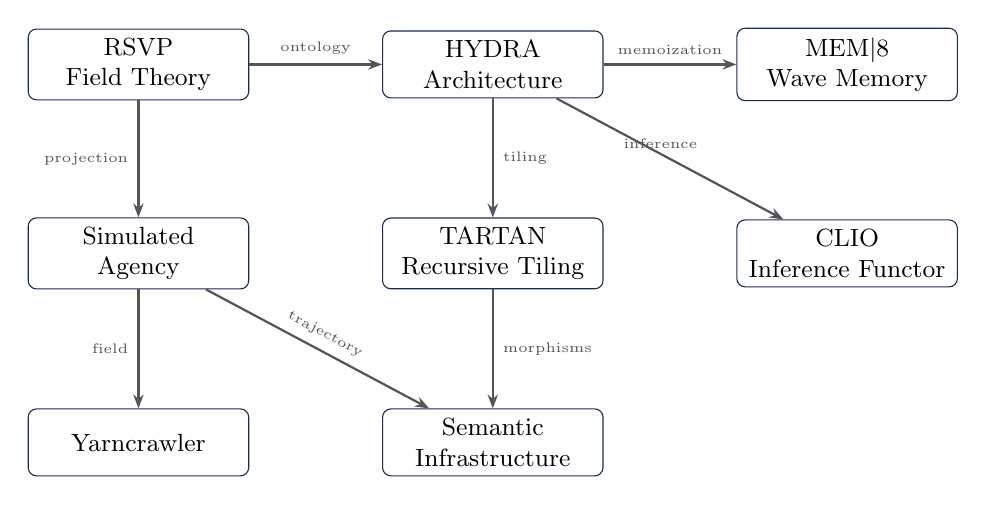
\begin{tikzpicture}[
  every node/.style={font=\small},
  box/.style={draw=rsvpblue, rounded corners=3pt, minimum width=2.8cm,
              minimum height=0.85cm, align=center, fill=white},
  arr/.style={-{Stealth[length=5pt]}, color=midgray, thick}
]
\node[box] (rsvp)        at (0, 0)    {RSVP\\Field Theory};
\node[box] (hydra)       at (4.5, 0)  {HYDRA\\Architecture};
\node[box] (tartan)      at (4.5,-2.4){TARTAN\\Recursive Tiling};
\node[box] (mem8)        at (9, 0)    {MEM\textbar8\\Wave Memory};
\node[box] (clio)        at (9,-2.4)  {CLIO\\Inference Functor};
\node[box] (simag)       at (0,-2.4)  {Simulated\\Agency};
\node[box] (seminfra)    at (4.5,-4.8){Semantic\\Infrastructure};
\node[box] (yarncrawler) at (0,-4.8)  {Yarncrawler};
\draw[arr] (rsvp)  -- (hydra)       node[midway,above]{\tiny ontology};
\draw[arr] (rsvp)  -- (simag)       node[midway,left]{\tiny projection};
\draw[arr] (hydra) -- (mem8)        node[midway,above]{\tiny memoization};
\draw[arr] (hydra) -- (tartan)      node[midway,right]{\tiny tiling};
\draw[arr] (hydra) -- (clio)        node[near start, below right]{\tiny inference};
\draw[arr] (tartan)-- (seminfra)    node[midway,right]{\tiny morphisms};
\draw[arr] (simag) -- (yarncrawler) node[midway,left]{\tiny field};
\draw[arr] (simag) -- (seminfra)    node[midway,above,sloped]{\tiny trajectory};
\end{tikzpicture}
\end{center}

%% ══════════════════════════════════════════════════════════
\section{Open Problems and Critical Assessment}
\label{sec:open}
%% ══════════════════════════════════════════════════════════

The framework makes falsifiable predictions. Hallucination rates should increase
with the topological complexity of the context category. Brittleness corresponds
to low $S$ in the trained model's manifold, predicting sharp out-of-distribution
degradation. Memory persistence scales logarithmically with initial excitation
strength relative to ambient entropy pressure, testable against forgetting curves
in biological or recurrent neural systems.

The following open problems are ordered by what they would unlock. Resolving
the first would underpin most of the theorems marked; the later problems
are important but more independent.

\emph{Regularity of RSVP equations} [first priority]. Under what conditions
do smooth initial data yield global classical solutions \citep{Tao2016}?
Unique continuation, which underpins the sheaf existence theorem and thus the
entire sheaf-theoretic semantics, depends on this. Singularity classification
--- whether singularities correspond to identifiable cognitive failure modes ---
is a secondary question.

\emph{Source term derivation.} The terms $\rho(v,S)$ and $\sigma(\Phi,v)$
in \eqref{eq:scalar}--\eqref{eq:entropy} are specified schematically. For
the language modeling domain, $\Phi$ might be identified with a coherence or
reward measure and $S$ with the entropy of the predictive distribution; for
the cognitive domain, with neural accessibility measures and population entropy.
Deriving $\rho$ and $\sigma$ from first principles in each domain is a
pre-condition for empirical testing.

\emph{Projection cohomology.} Compute $H^\bullet(\OpMan, \mathcal{F})$ and
interpret each group cognitively \citep{EdelsbrunnerHarer2010}. This requires
both the resolved regularity problem and domain-specific sheaf specifications.

\emph{Formalization of Conjecture~\ref{conj:universality}.} Precise definition
of $\mathbf{Adm}$ as a monoidal category and naturality verification in all
six domains \citep{EilenbergMacLane1945}.

\emph{Lean~4 verification.} Full proof of the admissibility preservation theorem
(Theorem~\ref{thm:ras}) without \texttt{sorry}; formal proof of the Minimal
Projection Theorem (Theorem~\ref{thm:minproj}).

\emph{Relation to existing literature.} The Free Energy Principle \citep{Friston2010}
corresponds approximately to minimizing $-\Phi + S$; RSVP subsumes FEP as a
special case when source terms encode the generative model structure, with the
additional contribution being Whitney stratification and sheaf coherence. The
relationship between IIT's integrated information and the RSVP accessibility
potential requires formal comparison. Sheaf neural networks (Hansen and Ghrist)
are the closest existing work; the main contribution of RSVP--HYDRA is
field-theoretic dynamics governing temporal evolution.

%% ══════════════════════════════════════════════════════════
\section{Conclusion}
%% ══════════════════════════════════════════════════════════

The conceptual center of this document is not the RSVP field equations,
the HYDRA architecture, or even the sheaf-theoretic formalism. It is the
following observation: meaning, memory, agency, cognition, social organization,
infrastructure, and cosmological structure can all be reformulated as problems
of preserving admissible future trajectories under irreversible projection.
Everything else in the document is a consequence or elaboration of that claim.

The claim is organized around the quartet $(\Traj, \ProjFam, \Adm, \Persist)$,
whose repeated specialization across domains gives the document its spine. The
Minimal Projection Theorem is the core established result. The RSVP field
equations are one way of giving that abstract structure dynamics. The stratified
manifold theory, sheaf semantics, categorical backbone, and political economy
sections are all specialized realizations of the same formal skeleton.

The framework's deepest contribution is the identification of admissibility
as relational. A state is not admissible in isolation; it is admissible relative
to a trajectory and a family of allowed continuations. This moves the framework
from object ontology to process ontology with consequences at every level.

The statement classification introduced in this version --- for established
mathematics, for framework definitions, for research conjectures ---
makes visible what was previously implied: that a substantial and important part
of the framework consists of research conjectures that organize future work
rather than established results. The Structural Universality Conjecture is the
largest of these; the regularity of the RSVP equations and the precise
specification of the semantic state sheaf are the most urgent.

That is where the framework is: a coherent theoretical program with a genuine
mathematical core, significant open problems, and a clear direction.

\bigskip
\noindent\rule{\textwidth}{0.4pt}


%% ══════════════════════════════════════════════════════════
%%  APPENDICES
%% ══════════════════════════════════════════════════════════
\clearpage
\appendix
\renewcommand{\thesection}{\Alph{section}}
\titleformat{\section}{\large\bfseries\color{accentgold}}{\appendixname~\thesection.}{0.8em}{}

\section{Mathematical Preliminaries}

Smooth manifolds, tangent bundles, Lie derivatives, and fiber bundles
follow \citet{Lee2013,Spivak1999}. A sheaf $\mathcal{F}$ on $X$ assigns to
each open $U$ an abelian group $\mathcal{F}(U)$ with restriction maps
satisfying identity and gluing axioms \citep{Godement1958}. Categories,
functors, and natural transformations follow \citet{MacLane1998}; monoidal
categories are taken in the standard sense \citep{MacLane1998}. Dependent
type systems and Curry--Howard follow \citet{CurryHoward}.

Notation: $\Traj$ denotes trajectory space, $\OpMan$ operational manifolds,
$\Adm$ admissibility structures, $\ProjFam = \{\pi_i\}$ projection families,
$A(x)$ admissible future sets, $\Real$ the realization map.

\section{RSVP Field Equations: Structural Properties}

\begin{theorem}[Admissibility Basin Existence]
For smooth, compactly supported initial data $(\Phi_0, v_0, S_0)$, the RSVP
system admits at least one local classical solution, and there exists a
forward-invariant open neighborhood $\Adm_0 \subset \Traj$ of the initial
configuration constituting an admissibility basin.
\end{theorem}

\begin{theorem}[Lyapunov Stability]
The persistence functional $\Persist = \int_\OpMan (|\Phi|^2 + |v|^2 + S)\,d\mathrm{vol}_g$
satisfies $\frac{d\Persist}{dt} \leq 0$ along solutions in the admissibility basin \citep{Arnold1989}.
\end{theorem}

\begin{proposition}[Entropy Monotonicity]
The entropy field satisfies $\partial S/\partial t \geq 0$ in regions where
$\sigma(\Phi,v) \geq 0$. Memory residues are regions where entropy production
is locally suppressed by strong field excitation $|\Phi| \gg \|\nabla S\|$.
\end{proposition}

\section{Projection Geometry}

\begin{theorem}[Projection Stability]
If $\pi : \Traj \to \OpMan$ is admissibility-preserving and the flow on
$\Traj$ is $\Adm$-contracting, then the induced flow on $\OpMan$ is
$\pi(\Adm)$-contracting. Projection does not create new instabilities.
\end{theorem}

\begin{proposition}[Fiber Preservation]
Semantic fibers $\pi^{-1}(m)$ are connected for all $m \in \OpMan$ if and only
if the admissibility structure $\Adm$ is path-connected within each fiber.
\end{proposition}

\begin{proposition}[Entropy as Admissible Future Volume]
Defining $S(x,t) = \log|A(x,t)|$, the entropy field satisfies the transport
equation \eqref{eq:entropy} with $\sigma$ encoding the rate at which the
system generates or destroys admissibility volume. Additivity holds under
product decompositions of $\Adm$ \citep{Cover2006}.
\end{proposition}

\section{Stratified Semantic Manifolds: Full Treatment}

The TARTAN tiling is constructed to be semantically coherent: $\Phi$ is
approximately constant within each tile, $v$ is approximately uniform, and
stratum assignment is constant. The noise annotation
$\eta(T) = (\mathrm{osc}(\Phi,T)^2 + \mathrm{osc}(v,T)^2)^{1/2}$ is the
RSVP entropy field $S$ evaluated at the tile level.

Admissible phase transitions are governed by the tangent-cone condition:
a trajectory $\gamma$ can cross from $S_\alpha$ to $S_\beta$ only if
$\gamma'(t) \in T_{\gamma(t_0)}S_\beta$ at the crossing \citep{Whitney1965,Mather1973}.
Non-admissible crossings produce semantic nulls. The Riemannian distance across
strata is $\mathrm{dist}_\OpMan(x,y) = \inf_\gamma \int_0^1 \|\dot\gamma(t)\|_{g_{\alpha(t)}}\,dt$
over admissible piecewise-smooth paths \citep{Lee2013}.

\section{Sheaf-Theoretic Semantics: Full Treatment}

The \v{C}ech cochain complex:
\begin{equation}
  C^0(\mathcal{U};\mathcal{F}) \xrightarrow{\delta^0} C^1(\mathcal{U};\mathcal{F})
  \xrightarrow{\delta^1} C^2(\mathcal{U};\mathcal{F}) \xrightarrow{\delta^2} \cdots
\end{equation}
has cohomology $H^k(\mathcal{U};\mathcal{F}) = \ker\delta^k/\mathrm{im}\,\delta^{k-1}$.
A 1-cocycle represents pairwise compatibility data; it is a coboundary if and
only if it is induced by globally consistent local sections. The group
$H^1(\OpMan,\mathcal{F})$ classifies all topologically stable patterns of
cognitive conflict \citep{Hatcher2002,Godement1958,KashiwaraSchapira1990}.

\section{Memory: Full Derivation}

The MEM\textbar8 wave packet realization of a memory state
$m = (\Phi_m, v_m, S_m)$ takes the form:
$\mathrm{Memory}_m = \mathrm{Wave}(A, \omega, \phi, D, I)$
where $A = \Phi_m$ (amplitude, scalar accessibility), $\omega$ encodes semantic
content, $\phi$ encodes the associative flow direction $v_m$, $D = e^{-S_m}$
is the decay factor (high-entropy memories decay faster), and $I$ is the
neighborhood interference term. Memory in MEM\textbar8 is active process, not
passive storage; retrieval is resonance, not indexing \citep{WilsonCowan1972}.

The Phoenix Protocol lifecycle is: Signal $\xrightarrow{\text{Marine}}$
$(s, \mathrm{Stable}(s)) \xrightarrow{\text{MEM\textbar8}}$
$(m, \mathrm{Resonant}(m)) \xrightarrow{\text{Heartbeat}}$
$(m', \mathrm{Persistent}(m')) \xrightarrow{\text{Rise}}$
$(r, \mathrm{Reconstructed}(r)) \xrightarrow{\text{Audit}}$
$(r, \mathrm{Coherent}(r))$.
Each arrow is a proof-carrying transformation; the chain realizes the dependent
type of the full HYDRA system \citep{CurryHoward}.

\section{Category Theory of HYDRA: Full Treatment}

\begin{theorem}[Compositionality]
The monoidal structure on $\mathbf{AdmSt}$ endows $H$ with compositional
semantics: the output of a composed HYDRA system equals the combination of
component outputs up to natural isomorphism \citep{EilenbergMacLane1945}.
\end{theorem}

\begin{proposition}[Admissibility Preservation Under Composition]
If each factor functor maps $\Adm$-morphisms to $\Adm$-morphisms, then $H$
is admissibility-preserving. The admissibility gate is closed under composition.
\end{proposition}

Any system realizing the same functor $H$ up to natural isomorphism is a
valid HYDRA implementation. Architecture-independence is a theorem, not an
assumption.

\section{Dependent Type Theory}

\begin{definition}[Admissible Type]
A type $\tau$ is admissible if every term $t : \tau$ carries a proof
$p_t : \mathrm{Admissible}(t)$ \citep{CurryHoward}.
\end{definition}

\begin{theorem}[Type Safety]
Well-typed HYDRA programs do not produce inadmissible states: if
$\Gamma \vdash t : \tau$ and $\tau$ is admissible, the result of evaluating
$t$ in any admissible context is admissible.
\end{theorem}

\begin{theorem}[Proof-Carrying Memoization, formal]
Cache entry $\hat t$ for input $x_0$ may be reused at input $x_1$ only when
a proof of $\mathrm{SameAdmissibilityFiber}(x_0, x_1)$ is available ---
certifying $\pi(x_0) = \pi(x_1)$. Since $A(x_0) = A(x_1)$ and $P(x,y)$
depends on $x$ only through $A(x)$, the certificate $p_0$ for $x_0$ is
valid for $x_1$ \citep{CurryHoward}.
\end{theorem}

\section{Semantic Fiber Bundles}

\begin{theorem}[Semantic Fiber Theorem]
Under mild regularity (specifically, that $\eta \in \mathcal{N}$ is a regular
value of $\Real$), the fiber $\Real^{-1}(\eta)$ is a smooth submanifold of
$\Theta$ of dimension $\dim\Theta - \dim\mathcal{N}$, by the regular level set
theorem \citep{Lee2013,Hatcher2002}.
\end{theorem}

The group of admissibility-preserving reparameterizations --- diffeomorphisms
$\psi : \Theta \to \Theta$ with $\Real(\psi(\theta)) = \Real(\theta)$ for all
$\theta$ --- acts on $\Theta$ by fiber-preserving diffeomorphisms, playing
the role of a gauge group \citep{BottTu1982}. A faithful theory of meaning must
be formulated in gauge-invariant quantities: those constant on fibers.

\section{Structural Universality}

\begin{definition}[Admissibility System]
$\mathcal{U} = (\Traj, \ProjFam, \Adm, \Persist)$ is an admissibility system.
These form a category $\mathbf{Adm}$ with admissibility-preserving functors
as morphisms \citep{MacLane1998}.
\end{definition}

The six target domains and their instantiations:

\begin{center}
\begin{tabular}{lll}
\toprule
\textbf{Domain} & $\Traj$ & \textbf{What persists} \\
\midrule
RSVP cosmology & plenum & field metastability \\
HYDRA cognition & cognitive trajectory space & admissible inference \\
MEM\textbar8 memory & wave state space & resonant field residue \\
Semantic Infrastructure & module dependency graphs & homotopy-compatible merges \\
Yarncrawler infrastructure & wear-dynamics phase space & entropy-bounded maintenance \\
Political economy & agent strategy space & collective admissibility \\
\bottomrule
\end{tabular}
\end{center}

Proving Conjecture~\ref{conj:universality} requires: (1) precise definition
of $\mathbf{Rep}$; (2) construction of $T$ on morphisms; (3) verification of
naturality in each domain; (4) proof that $T$ preserves admissibility-basin
structure \citep{EilenbergMacLane1945,MacLane1998}. These are the central
open problems.

\section{Engineering Realization: Module Correspondence}

\begin{center}
\begin{tabular}{lll}
\toprule
\textbf{Module} & \textbf{Theoretical correlate} & \textbf{Complexity} \\
\midrule
\texttt{admissibility} & admissibility gate & $O(|\Adm|)$ per transition \\
\texttt{wave\_field} & RSVP scalar-vector state machine & $O(N)$ per field step \\
\texttt{entropy} & entropy dissipation ($\sigma$ update) & $O(N)$ per step \\
\texttt{resonance} & resonance retrieval (MEM\textbar8 layer) & $O(\rho^{-\alpha}\log N)$ \\
\texttt{tartan} & recursive semantic tiling & $O(N\log N)$ \\
\texttt{projection} & semantic equivalence quotient & $O(N^2)$ worst case \\
\bottomrule
\end{tabular}
\end{center}

\section{Open Problems}

\emph{Global regularity.} Under what conditions do smooth initial data yield
global classical solutions to the RSVP equations \citep{Tao2016}? Do
singularities correspond to identifiable cognitive failure modes?

\emph{Projection cohomology.} Compute $H^\bullet(\OpMan, \mathcal{F})$ and
interpret each cohomology group cognitively \citep{EdelsbrunnerHarer2010}.

\emph{Semantic singularities.} Classify stratum boundary singularities following
\citet{Mather1973}; build a dictionary between Whitney singularity types and
cognitive phenomena.

\emph{Topological agency invariants.} Are there invariants of HYDRA systems
preserved under homotopy equivalence of $\OpMan$? \citep{Ghrist2014}

\emph{Derived-stack semantics.} Replace ordinary fibers with derived fibers
encoding higher coherence data \citep{Lurie2009}.

\emph{Neural implementations of resonance retrieval.} Connect the resonance
retrieval theorem to empirical measurements of neural oscillatory dynamics,
building on \citet{WilsonCowan1972}.

\emph{Full categorical formalization.} Prove Conjecture~\ref{conj:universality}
in the precise sense of \citet{EilenbergMacLane1945,MacLane1998}.

%% ══════════════════════════════════════════════════════════
\clearpage
\begin{thebibliography}{99}

\bibitem[Ambrose \& Singer(1953)]{AmbroseSinger1953}
W. Ambrose and I. M. Singer, A theorem on holonomy,
\textit{Transactions of the American Mathematical Society}, 75(3):428--443, 1953.

\bibitem[Arnold(1989)]{Arnold1989}
V. I. Arnold, \textit{Mathematical Methods of Classical Mechanics}, 2nd ed., Springer, 1989.

\bibitem[Bellman(1957)]{Bellman1957}
R. Bellman, \textit{Dynamic Programming}, Princeton University Press, 1957.

\bibitem[Bott \& Tu(1982)]{BottTu1982}
R. Bott and L. W. Tu, \textit{Differential Forms in Algebraic Topology}, Springer, 1982.

\bibitem[Cover \& Thomas(2006)]{Cover2006}
T. M. Cover and J. A. Thomas, \textit{Elements of Information Theory}, 2nd ed., Wiley, 2006.

\bibitem[Curry \& Feys(1958)]{CurryHoward}
H. B. Curry and R. Feys, \textit{Combinatory Logic}, North-Holland, 1958.

\bibitem[Edelsbrunner \& Harer(2010)]{EdelsbrunnerHarer2010}
H. Edelsbrunner and J. Harer, \textit{Computational Topology: An Introduction},
American Mathematical Society, 2010.

\bibitem[Eilenberg \& Mac Lane(1945)]{EilenbergMacLane1945}
S. Eilenberg and S. Mac Lane, General theory of natural equivalences,
\textit{Transactions of the American Mathematical Society}, 58(2):231--294, 1945.

\bibitem[Friston(2010)]{Friston2010}
K. Friston, The free-energy principle: a unified brain theory?,
\textit{Nature Reviews Neuroscience}, 11(2):127--138, 2010.

\bibitem[Ghrist(2014)]{Ghrist2014}
R. Ghrist, \textit{Elementary Applied Topology}, Createspace, 2014.

\bibitem[Godement(1958)]{Godement1958}
R. Godement, \textit{Topologie Alg\'{e}brique et Th\'{e}orie des Faisceaux},
Hermann, Paris, 1958.

\bibitem[Hatcher(2002)]{Hatcher2002}
A. Hatcher, \textit{Algebraic Topology}, Cambridge University Press, 2002.

\bibitem[Kashiwara \& Schapira(1990)]{KashiwaraSchapira1990}
M. Kashiwara and P. Schapira, \textit{Sheaves on Manifolds}, Springer, 1990.

\bibitem[Lee(2013)]{Lee2013}
J. M. Lee, \textit{Introduction to Smooth Manifolds}, 2nd ed., Springer, 2013.

\bibitem[Lurie(2009)]{Lurie2009}
J. Lurie, \textit{Higher Topos Theory}, Princeton University Press, 2009.

\bibitem[Mac Lane(1998)]{MacLane1998}
S. Mac Lane, \textit{Categories for the Working Mathematician}, 2nd ed., Springer, 1998.

\bibitem[Mather(1973)]{Mather1973}
J. N. Mather, Stratifications and mappings,
in \textit{Dynamical Systems}, Academic Press, 1973.

\bibitem[Milnor(1963)]{Milnor1963}
J. Milnor, \textit{Morse Theory}, Princeton University Press, 1963.

\bibitem[Pearl(2009)]{Pearl2009}
J. Pearl, \textit{Causality}, 2nd ed., Cambridge University Press, 2009.

\bibitem[Rudin(1991)]{Rudin1991}
W. Rudin, \textit{Functional Analysis}, 2nd ed., McGraw-Hill, 1991.

\bibitem[Sandel(2020)]{Sandel2020}
M. J. Sandel, \textit{The Tyranny of Merit: What's Become of the Common Good?},
Farrar, Straus and Giroux, 2020.

\bibitem[Spivak(1999)]{Spivak1999}
M. Spivak, \textit{A Comprehensive Introduction to Differential Geometry},
Publish or Perish, 1999.

\bibitem[Tao(2006)]{Tao2016}
T. Tao, \textit{Nonlinear Dispersive Equations: Local and Global Analysis},
American Mathematical Society, 2006.

\bibitem[Tenenbaum et al.(2000)]{TenenbaumSilvaLangford2000}
J. B. Tenenbaum, V. de Silva, and J. C. Langford,
A global geometric framework for nonlinear dimensionality reduction,
\textit{Science}, 290(5500):2319--2323, 2000.

\bibitem[Whitney(1965)]{Whitney1965}
H. Whitney, Tangents to an analytic variety,
\textit{Annals of Mathematics}, 81(3):496--549, 1965.

\bibitem[Wilson \& Cowan(1972)]{WilsonCowan1972}
H. R. Wilson and J. D. Cowan,
Excitatory and inhibitory interactions in localized populations of model neurons,
\textit{Biophysical Journal}, 12(1):1--24, 1972.

\bibitem[Zhang et al.(2020)]{ZhangEtAl2020}
M. Zhang, Z. Cui, M. Neumann, and Y. Chen,
An end-to-end deep learning architecture for graph classification,
\textit{AAAI}, 2020.

\end{thebibliography}

\end{document}
